\chapter{Функции обработчика прерывания от системного таймера}

\section{ОС семейства Unix}

\subsection{По тику}

В задачи обработчика прерывания от системного таймера по тику входит:

\begin{itemize}
	\item инкремент счетчика времени с момента запуска системы (SVR4);
	\item инкремент счетчика реального времени;
	\item декремент кванта;
	\item декремент счетчиков времени и при достижении счетчиками нуля установка флага для обработчиков отложенных вызовов;
	\item инкремент счетчика процессорного времени, полученного процессом в режиме задачи и в режиме ядра.
\end{itemize}

\subsection{По главному тику}

В задачи обработчика прерывания от системного таймера по главному тику входит:

\begin{itemize}
	\item инициализация отложенного вызова функции планировщика;
	\item инициализация отложенного вызова процедуры \textit{wakeup}, которая меняет состояние процесса с <<спящего>> на <<готовый к выполнению>>;
	\item пробуждение системных процессов, таких как \textit{swapper} и \textit{pagedaemon};
	\item декремент счетчика времени, которое осталось до отправления одного из следующих сигналов:
	\begin{itemize}
		\item \textit{SIGALRM} - сигнал, посылаемый процессу по истечении промежутка реального времени;
		\item \textit{SIGPROF} - сигнал, посылаемый процессу по истечении времени, которое задано в таймере профилирования;
		\item \textit{SIGVTALRM} - сигнал, посылаемый процессу по истечении времени, которое задано в ''виртуальном'' таймере.
	\end{itemize}
\end{itemize}

\subsection{По кванту}

Обработчик прерывания от системного таймера по кванту посылает сигнал \textit{SIGXCPU} текущему процессу, если он превысил выделенную для него квоту процессорного времени.

\section{ОС семейства Windows}

\subsection{По тику}

В задачи обработчика прерывания от системного таймера по тику входит:

\begin{itemize}
	\item инкремент счетчика реального времени;
	\item декремент кванта текущего потока;
	\item декремент счетчиков отложенных задач.
\end{itemize}

\subsection{По главному тику}

Обработчик прерывания от системного таймера по главному тику инициализирует диспетчер настройки баланса, освобождая объект "событие"{}, на котором он ожидает.

\subsection{По кванту}

Обработчик прерывания от системного таймера по кванту инициализирует диспетчеризацию потоков путем постановки соответствующего объекта в очередь DPC.

\chapter{Пересчет динамических приоритетов}

Системы семейств Unix и Windows являются системами разделения времени с динамическими приоритетами и вытеснением. Динамические приоритеты могут иметь только пользовательские процессы.

\section{ОС семейства Unix}

При создании процесса ему назначается базовый приоритет.
Очередь процессов, готовых к выполнению, формируется согласно приоритетам процессов и принципу вытесняющего циклического планирования. В первую очередь выполняются процессы, имеющие больший приоритет. Процессы с одинаковыми приоритетами выполняются циклически друг за другом, в течение кванта времени. В случае, если процесс с более высоким приоритетом поступает в очередь готовых к выполнению процессов, планировщик вытесняет текущий процесс и предоставляет ресурс более приоритетному процессу.

Приоритет задается целым числом из диапазона от 0 до 127. Чем меньше число, тем выше приоритет процесса. Приоритеты от 0 до 49 зарезервированы ядром опреационной системы, в связи с чем пользовательские процессы могут обладать приоритетом от 50 до 127.

В отличие от приоритетов ядра, являющихся фиксированными величинами, приоритеты пользовательских процессов могут изменяться во времени в зависимости от двух факторов:

\begin{itemize}
	\item фактор любезности. Чем меньше его значение, тем выше приоритет процесса. Фактор любезности может быть изменен с помощью системного вызова \textit{nice}, однако только суперпользователь может увеличивать значение приоритета;
	\item фактор использования, который определяется степенью последней загруженности CPU процессом.
\end{itemize}

Дескриптор процесса \textit{proc} содержит следующие поля, относящиеся к приоритету:
\begin{itemize}
    \item \textit{p\_pri} – текущий приоритет планирования;
    \item \textit{p\_usrpri} – приоритет процесса в режиме задачи;
    \item \textit{p\_cpu} – результат последнего измерения степени загруженности процессора процессом;
    \item \textit{p\_nice} – фактор любезности.
\end{itemize}

Планировщик использует значение \textit{p\_pri} для принятия решения о том, какой процесс направить на выполнение. У процесса, который находится в режиме задачи, значения \textit{p\_pri} и \textit{p\_usrpri} равны. Значение текущего приоритета \textit{p\_pri} может быть повышено планировщиком для выполнения процесса в режиме ядра (\textit{p\_usrpri} будет использоваться для хранения приоритета, который будет назначен при возврате в режим задачи).

Ядро системы связывает приоритет сна с событием или ожидаемым ресурсом, из-за которого процесс может блокироваться. Когда процесс ''просыпается'' после
блокировки, ядро устанавливает в поле \textit{p\_pri} приоритет сна --- значение приоритета из диапазона от 0 до 49, зависящее от события или ресурса по которому произошла блокировка. Значения приоритетов сна для событий в системе \textit{4.3BSD} описаны в таблице \ref{tbl:bsd}.

\begin{table}[H]
    \begin{center}
        \begin{threeparttable}
        \captionsetup{justification=raggedright,singlelinecheck=off}
        \caption{Приоритеты сна в 4.3BSD}
        \label{tbl:bsd}
        \begin{tabular}{|c|c|c|}
            \hline
            Приоритет & Значение & Описание \\
            \hline
            PSWP & 0 & Свопинг \\ \hline  
            PSWP + 1 & 1 & Страничный демон \\ \hline
            PSWP + 1/2/4 & 1/2/4 & Другие действия при обработке памяти \\ \hline
            PINOD & 10 & Ожидание освобождения inode  \\ \hline 
            PRIBIO & 20 & Ожидание дискового ввода-вывода \\ \hline
            PRIBIO + 1 & 21 & Ожидание освобождения буфера \\ \hline
            PZERO & 25 & Базовый приоритет \\ \hline
            TTIPRI & 28 & Ожидание ввода с терминала \\ \hline
            TTORPI & 29 & Ожидание вывода с терминала \\ \hline
            PWAIT & 30 & Ожидание завершения процесса потомка \\ \hline
            PLOCK & 35 & $\begin{array}{cccc}
            	$Консультативное ожидание$ \\
            	$блокированного ресурса$
            \end{array} $   \\ \hline
            PSLEP & 40 & Ожидание сигнала \\ \hline                                             
		\end{tabular}
    \end{threeparttable}
\end{center}
\end{table}

При инициализации процесса поле \textit{p\_cpu} равно нулю. На каждом тике обработчик прерывания увеличивает поле \textit{p\_cpu} текущего процесса на единицу, до максимального значения, равного 127. Каждую секунду, обработчик прерывания инициализирует отложенный вызов процедуры \textit{schedcpu()}, которая уменьшает значение \textit{p\_cpu} каждого процесса исходя из фактора ''полураспада''.

Для расчёта фактора полураспада применяется формула
\eqref{for:bsd}.

\begin{equation}
    \label{for:bsd}
    decay = \frac{2 \cdot load\_average}{2 \cdot load\_average + 1}
\end{equation}

где \textit{load\_average} - это среднее количество процессов, находящихся в состоянии готовности к выполнению, за последнюю секунду.

Процедура \textit{schedcpu()} пересчитывает приоритеты для режима задачи всех процессов по формуле \eqref{for:task}.

\begin{equation}
    \label{for:task}
    p\_usrpri = PUSER + \frac{p\_cpu}{2} + 2 \cdot p\_nice
\end{equation}

где \textit{PUSER} - базовый приоритет в режиме задачи, равный 50.

В результате \textit{p\_cpu} будет увеличен, если процесс до вытеснения другим процессом использовал большое количество процессорного времени. Это приведет к росту значения \textit{p\_usrpri} и, следовательно, к понижению приоритета. Чем дольше процесс простаивает в очереди на выполнение, тем больше фактор
полураспада уменьшает его \textit{p\_cpu}. Такая схема предотвращает бесконечное откладывание низкоприоритетных процессов в ОС.


\section{ОС семейства Windows}

В Windows процессу при создании назначается базовый приоритет. В Windows реализовано вытесняющее планирование на основе уровней приоритета: если поток с более высоким приоритетом становится готовым к выполнению, поток с более низким приоритетом вытесняется планировщиком, даже если квант текущего не истек. По истечению кванта времени текущего потока, ресурс передается самому приоритетному потоку в очереди готовых к выполнению.

В Windows \textit{диспетчер настройки баланса} раз в секунду сканирует очередь готовых потоков. Если обнаружены потоки, ожидающие выполнения более 4 секунд, диспетчер настройки баланса повышает их приоритет до 15. Когда истекает квант, приоритет потока снижается до базового приоритета. Если поток не был завершен за квант времени или был вытеснен потоком с более высоким приоритетом, то после снижения приоритета поток возвращается в очередь.

Для того, чтобы минимизировать расход процессорного времени, диспетчер настройки баланса сканирует только 16 попозиций в очереди и повышает приоритет не более чем у 10 потоков за один проход. При обнаружении 10 потоков, приоритет которых следует повысить, диспетчер настройки баланса прекращает сканирование. При следующем проходе сканирование возобновляется с того места, где оно было прервано.

В Windows используется 32 уровня приоритета:
\begin{itemize}
    \item от 0 до 15 - динамические уровни (уровень 0 зарезервирован для потока обнуления страниц);
    \item от 16 до 31 - приоритеты процессов реального времени (31 --- наивысший).
\end{itemize}

Уровни приоритета потоков назначаются с дыух позиций: Windows API и ядра ОС.

Сначала Windows API сортирует процессы по классу приоритета, которые были назначены при их создании:
\begin{itemize}
    \item реального времени (Real-time) - (4);
    \item высокий (High) - (3);
    \item выше обычного (Above Normal) - (6);
    \item обычный (Normal) - (2);
    \item ниже обычного (Below Normal) - (5);
    \item простой (Idle) - (1).
\end{itemize}

Затем назначается относительный приоритет потоков процесса:
\begin{itemize}
    \item критичный по времени (Time-critical) - (15);
    \item наивысший (Highest) - (2);
    \item выше обычного (Above-normal) - (1);
    \item обычный (Normal) - (0);
    \item ниже обычного (Below-normal) - (–1);
    \item низший (Lowest) - (–2);
    \item простой (Idle) - (–15)
\end{itemize}

В таблице \ref{tab:prioritet} показано соответствие между приоритетами Windows API и ядра системы.

\begin{table}[H]
    \caption{Соответствие между приоритетами Windows API и ядра Windows}
    \begin{center}
        \begin{tabular}{|c|c|c|c|c|c|c|}
            \hline
            Класс приоритета & Real-time & High & Above &
            Normal & Below Normal & Idle \\ \hline
            Time Critical & 31 & 15 & 15 & 15 & 15 & 15 \\ \hline
            Highest & 26 & 15 & 12 & 10 & 8 & 6 \\ \hline
            Above Normal & 25 & 14 & 11 & 9 & 7 & 5 \\ \hline
            Normal & 24 & 13 & 10 & 8 & 6 & 4 \\ \hline
            Below Normal & 23 & 12 & 9 & 7 & 5 & 3 \\ \hline
            Lowest & 22 & 11 & 8 & 6 & 4 & 2 \\ \hline
            Idle & 16 & 1 & 1 & 1 & 1 & 1 \\ \hline
        \end{tabular}
    \end{center}
    \label{tab:prioritet}
\end{table}

Планировщик может повысить текущий приоритет потока в динамическом диапазоне (от 1 до 15) по следующим причинам:

\begin{itemize}
    \item повышение вследствие событие планировщика или диспетчера;
    \item повышение приоритета владельца блокировки;
    \item завершение операций ввода/вывода (таблица \ref{tab:input-output});
    
\begin{table}[H]
    \caption{Рекомендуемые значения повышения приоритета}
    \begin{center}
        \begin{tabular}{|p{100mm}|l|}
            \hline
            \textbf{Устройство} & \textbf{Приращение} \\\hline
            Диск, CD-ROM, параллельный порт, видео & 1 \\ \hline
            Сеть, почтовый ящик, именованный канал, последовательный порт & 2 \\ \hline
            Клавиатура, мышь & 6 \\ \hline
            Звуковая плата & 8 \\ \hline
        \end{tabular}
    \end{center}
    \label{tab:input-output}
\end{table}
    \item ввод из пользовательского интерфейса;
    \item длительное ожидание ресурса исполняющей системы;
    \item ожидание объекта ядра;
    \item готовый к выполнению поток не был запущен в течение длительного времени;
    \item повышение приоритета службой планировщика MMCSS.
\end{itemize}

\subsection{MMCSS}

Для того, чтобы потоки, на которых выполняются различные мультимедийные приложения могли выполняться с минимальными задержками, драйвур \textit{MMCSS} (\textit{MultiMedia Class Scheduler Service}) временно повышает приоритет таких потоков.

MMCSS работает со следующими задачами:

\begin{itemize}
	\item звук;
	\item возможность использования функции записи;
	\item воспроизведение звукового или видео контента;
	\item аудио профессионального качества;
	\item задачи администратора многооконного режима.
\end{itemize}

Одно из наиболее важных свойств для планирования потоков --- категория планирования (Scheduling Category) --- первичный фактор определяющий приоритет потоков, зарегестрированных в MMCSS (таблица \ref{tab:category}).

\begin{table}[H]
    \caption{Категории планирования}
    \begin{center}
        \begin{tabular}{|p{40mm}|p{30mm}|p{80mm}|}
            \hline
            \textbf{Категория} & \textbf{Приоритет} & \textbf{Описание} \\
            \hline
            High (Высокая) & 23-26 & Потоки профессионального аудио (Pro
Audio), запущенные с приоритетом выше, чем у других потоков на системе, за
исключением критических системных потоков \\
            \hline
            Medium (Средняя) & 16-22 & Потоки, являющиеся частью приложений
первого плана, например Windows Media Player \\
            \hline
            Low (Низкая) & 8-15 & Все остальные потоки, не являющиеся частью
предыдущих категорий \\
            \hline
            Exhausted (Исчерпавших потоков) & 1-7 & Потоки, исчерпавшие свою
долю времени центрального процессора, выполнение которых продолжиться, только
если не будут готовы к выполнению другие потоки с более высоким уровнем
приоритета \\
            \hline
        \end{tabular}
    \end{center}
    \label{tab:category}
\end{table}

Функции MMCSS временно повышают приоритет потоков, зарегестрированных с MMCSS до уровня, соответствующего их категориям планирования. Затем их приоритет снижается до уровня, соответствующего категории \textit{Exhausted} для того, чтобы другие потоки могли получить ресурс.

\subsection{Уровни запросов прерываний}

Хотя контроллеры прерываний устанавливают приоритетность прерываний,
Windows устанавливает свою собственную схему приоритетности прерываний, известную как уровни запросов прерываний (IRQL). В ядре IRQL-уровни представлены в виде номеров от 0 до 31 на системах x86, где более высоким номерам соответствуют прерывания с более высоким приоритетом.

На рис. \ref{img:irql} показаны IRQL-уровни для архитектуры x86.

\begin{figure}[H]
	\begin{center}
		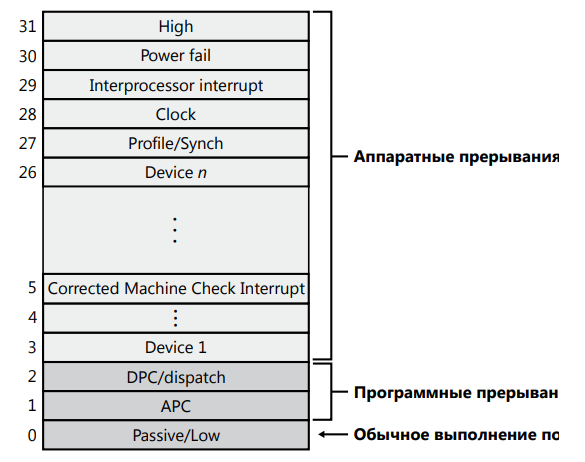
\includegraphics[scale=0.9]{img/irql.png}
	\end{center}
	\captionsetup{justification=centering}
	\caption{Уровни запросов прерываний}
	\label{img:irql}
\end{figure}

Прерывания обслуживаются в порядке их приоритета, и прерывания с более
высоким уровнем приоритета получают преимущество в обслуживании. При
возникновении прерывания с высоким уровнем приоритета процессор сохраняет состояние прерванного потока и запускает связанный с прерыванием диспетчер системных прерываний. 

